\documentclass[1p]{elsarticle_modified}
%\bibliographystyle{elsarticle-num}

%\usepackage[colorlinks]{hyperref}
%\usepackage{abbrmath_seonhwa} %\Abb, \Ascr, \Acal ,\Abf, \Afrak
\usepackage{amsfonts}
\usepackage{amssymb}
\usepackage{amsmath}
\usepackage{amsthm}
\usepackage{scalefnt}
\usepackage{amsbsy}
\usepackage{kotex}
\usepackage{caption}
\usepackage{subfig}
\usepackage{color}
\usepackage{graphicx}
\usepackage{xcolor} %% white, black, red, green, blue, cyan, magenta, yellow
\usepackage{float}
\usepackage{setspace}
\usepackage{hyperref}

\usepackage{tikz}
\usetikzlibrary{arrows}

\usepackage{multirow}
\usepackage{array} % fixed length table
\usepackage{hhline}

%%%%%%%%%%%%%%%%%%%%%
\makeatletter
\renewcommand*\env@matrix[1][\arraystretch]{%
	\edef\arraystretch{#1}%
	\hskip -\arraycolsep
	\let\@ifnextchar\new@ifnextchar
	\array{*\c@MaxMatrixCols c}}
\makeatother %https://tex.stackexchange.com/questions/14071/how-can-i-increase-the-line-spacing-in-a-matrix
%%%%%%%%%%%%%%%

\usepackage[normalem]{ulem}

\newcommand{\msout}[1]{\ifmmode\text{\sout{\ensuremath{#1}}}\else\sout{#1}\fi}
%SOURCE: \msout is \stkout macro in https://tex.stackexchange.com/questions/20609/strikeout-in-math-mode

\newcommand{\cancel}[1]{
	\ifmmode
	{\color{red}\msout{#1}}
	\else
	{\color{red}\sout{#1}}
	\fi
}

\newcommand{\add}[1]{
	{\color{blue}\uwave{#1}}
}

\newcommand{\replace}[2]{
	\ifmmode
	{\color{red}\msout{#1}}{\color{blue}\uwave{#2}}
	\else
	{\color{red}\sout{#1}}{\color{blue}\uwave{#2}}
	\fi
}

\newcommand{\Sol}{\mathcal{S}} %segment
\newcommand{\D}{D} %diagram
\newcommand{\A}{\mathcal{A}} %arc


%%%%%%%%%%%%%%%%%%%%%%%%%%%%%5 test

\def\sl{\operatorname{\textup{SL}}(2,\Cbb)}
\def\psl{\operatorname{\textup{PSL}}(2,\Cbb)}
\def\quan{\mkern 1mu \triangleright \mkern 1mu}

\theoremstyle{definition}
\newtheorem{thm}{Theorem}[section]
\newtheorem{prop}[thm]{Proposition}
\newtheorem{lem}[thm]{Lemma}
\newtheorem{ques}[thm]{Question}
\newtheorem{cor}[thm]{Corollary}
\newtheorem{defn}[thm]{Definition}
\newtheorem{exam}[thm]{Example}
\newtheorem{rmk}[thm]{Remark}
\newtheorem{alg}[thm]{Algorithm}

\newcommand{\I}{\sqrt{-1}}
\begin{document}

%\begin{frontmatter}
%
%\title{Boundary parabolic representations of knots up to 8 crossings}
%
%%% Group authors per affiliation:
%\author{Yunhi Cho} 
%\address{Department of Mathematics, University of Seoul, Seoul, Korea}
%\ead{yhcho@uos.ac.kr}
%
%
%\author{Seonhwa Kim} %\fnref{s_kim}}
%\address{Center for Geometry and Physics, Institute for Basic Science, Pohang, 37673, Korea}
%\ead{ryeona17@ibs.re.kr}
%
%\author{Hyuk Kim}
%\address{Department of Mathematical Sciences, Seoul National University, Seoul 08826, Korea}
%\ead{hyukkim@snu.ac.kr}
%
%\author{Seokbeom Yoon}
%\address{Department of Mathematical Sciences, Seoul National University, Seoul, 08826,  Korea}
%\ead{sbyoon15@snu.ac.kr}
%
%\begin{abstract}
%We find all boundary parabolic representation of knots up to 8 crossings.
%
%\end{abstract}
%\begin{keyword}
%    \MSC[2010] 57M25 
%\end{keyword}
%
%\end{frontmatter}

%\linenumbers
%\tableofcontents
%
\newcommand\colored[1]{\textcolor{white}{\rule[-0.35ex]{0.8em}{1.4ex}}\kern-0.8em\color{red} #1}%
%\newcommand\colored[1]{\textcolor{white}{ #1}\kern-2.17ex	\textcolor{white}{ #1}\kern-1.81ex	\textcolor{white}{ #1}\kern-2.15ex\color{red}#1	}

{\Large $\underline{10_{144}~(K10n_{28})}$}

\setlength{\tabcolsep}{10pt}
\renewcommand{\arraystretch}{1.6}
\vspace{1cm}\begin{tabular}{m{100pt}>{\centering\arraybackslash}m{274pt}}
\multirow{5}{120pt}{
	\centering
	\includegraphics[width=112pt]{../../../GIT/diagram.site/Diagrams/png/228_10_144.png}\\
\ \ \ A knot diagram\footnotemark}&
\allowdisplaybreaks
\textbf{Linearized knot diagam} \\
\cline{2-2}
 &
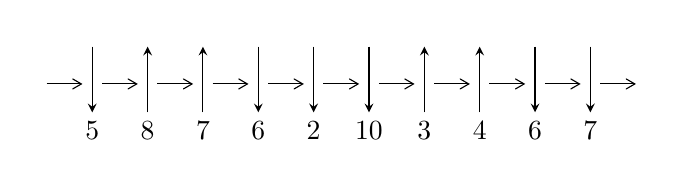
\begin{tikzpicture}[x=20pt, y=17pt]
	% nodes
	\node (C0) at (0, 0) {};
	\node (C1) at (1, 0) {};
	\node (C1U) at (1, +1) {};
	\node (C1D) at (1, -1) {5};

	\node (C2) at (2, 0) {};
	\node (C2U) at (2, +1) {};
	\node (C2D) at (2, -1) {8};

	\node (C3) at (3, 0) {};
	\node (C3U) at (3, +1) {};
	\node (C3D) at (3, -1) {7};

	\node (C4) at (4, 0) {};
	\node (C4U) at (4, +1) {};
	\node (C4D) at (4, -1) {6};

	\node (C5) at (5, 0) {};
	\node (C5U) at (5, +1) {};
	\node (C5D) at (5, -1) {2};

	\node (C6) at (6, 0) {};
	\node (C6U) at (6, +1) {};
	\node (C6D) at (6, -1) {10};

	\node (C7) at (7, 0) {};
	\node (C7U) at (7, +1) {};
	\node (C7D) at (7, -1) {3};

	\node (C8) at (8, 0) {};
	\node (C8U) at (8, +1) {};
	\node (C8D) at (8, -1) {4};

	\node (C9) at (9, 0) {};
	\node (C9U) at (9, +1) {};
	\node (C9D) at (9, -1) {6};

	\node (C10) at (10, 0) {};
	\node (C10U) at (10, +1) {};
	\node (C10D) at (10, -1) {7};
	\node (C11) at (11, 0) {};

	% arrows
	\draw[->,>={angle 60}]
	(C0) edge (C1) (C1) edge (C2) (C2) edge (C3) (C3) edge (C4) (C4) edge (C5) (C5) edge (C6) (C6) edge (C7) (C7) edge (C8) (C8) edge (C9) (C9) edge (C10) (C10) edge (C11) ;	\draw[->,>=stealth]
	(C1U) edge (C1D) (C2D) edge (C2U) (C3D) edge (C3U) (C4U) edge (C4D) (C5U) edge (C5D) (C6U) edge (C6D) (C7D) edge (C7U) (C8D) edge (C8U) (C9U) edge (C9D) (C10U) edge (C10D) ;
	\end{tikzpicture} \\
\hhline{~~} \\& 
\textbf{Solving Sequence} \\ \cline{2-2} 
 &
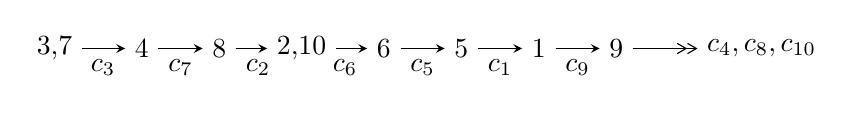
\begin{tikzpicture}[x=28pt, y=7pt]
	% node
	\node (A0) at (-1/8, 0) {3,7};
	\node (A1) at (1, 0) {4};
	\node (A2) at (2, 0) {8};
	\node (A3) at (49/16, 0) {2,10};
	\node (A4) at (33/8, 0) {6};
	\node (A5) at (41/8, 0) {5};
	\node (A6) at (49/8, 0) {1};
	\node (A7) at (57/8, 0) {9};
	\node (C1) at (1/2, -1) {$c_{3}$};
	\node (C2) at (3/2, -1) {$c_{7}$};
	\node (C3) at (5/2, -1) {$c_{2}$};
	\node (C4) at (29/8, -1) {$c_{6}$};
	\node (C5) at (37/8, -1) {$c_{5}$};
	\node (C6) at (45/8, -1) {$c_{1}$};
	\node (C7) at (53/8, -1) {$c_{9}$};
	\node (A8) at (9, 0) {$c_{4},c_{8},c_{10}$};

	% edge
	\draw[->,>=stealth]	
	(A0) edge (A1) (A1) edge (A2) (A2) edge (A3) (A3) edge (A4) (A4) edge (A5) (A5) edge (A6) (A6) edge (A7) ;
	\draw[->>,>={angle 60}]	
	(A7) edge (A8);
\end{tikzpicture} \\ 

\end{tabular} \\

\footnotetext{
The image of knot diagram is generated by the software ``\textbf{Draw programme}" developed by Andrew Bartholomew(\url{http://www.layer8.co.uk/maths/draw/index.htm\#Running-draw}), where we modified some parts for our purpose(\url{https://github.com/CATsTAILs/LinksPainter}).
}\phantom \\ \newline 
\centering \textbf{Ideals for irreducible components\footnotemark of $X_{\text{par}}$} 
 
\begin{align*}
I^u_{1}&=\langle 
u^8-2 u^7+5 u^6-6 u^5+7 u^4-5 u^3+3 u^2+b-2 u+1,\\
\phantom{I^u_{1}}&\phantom{= \langle  }u^9- u^8+5 u^7-4 u^6+8 u^5-5 u^4+3 u^3-2 u^2+2 a-2 u,\\
\phantom{I^u_{1}}&\phantom{= \langle  }u^{10}-3 u^9+9 u^8-16 u^7+24 u^6-27 u^5+23 u^4-16 u^3+8 u^2-4 u+2\rangle \\
I^u_{2}&=\langle 
u^4 a+u^3 a- u^4+2 u^2 a- u^3+a u-2 u^2+b- a- u,\;- u^5- u^4+u^2 a-4 u^3+a^2-3 u^2+a-4 u-2,\\
\phantom{I^u_{2}}&\phantom{= \langle  }u^6+u^5+3 u^4+2 u^3+2 u^2+u-1\rangle \\
I^u_{3}&=\langle 
b+2 u-1,\;2 a+u,\;u^2+2\rangle \\
\\
I^v_{1}&=\langle 
a,\;b+1,\;v+1\rangle \\
\end{align*}
\raggedright * 4 irreducible components of $\dim_{\mathbb{C}}=0$, with total 25 representations.\\
\footnotetext{All coefficients of polynomials are rational numbers. But the coefficients are sometimes approximated in decimal forms when there is not enough margin.}
\newpage
\renewcommand{\arraystretch}{1}
\centering \section*{I. $I^u_{1}= \langle u^8-2 u^7+\cdots+b+1,\;u^9- u^8+\cdots+2 a-2 u,\;u^{10}-3 u^9+\cdots-4 u+2 \rangle$}
\flushleft \textbf{(i) Arc colorings}\\
\begin{tabular}{m{7pt} m{180pt} m{7pt} m{180pt} }
\flushright $a_{3}=$&$\begin{pmatrix}1\\0\end{pmatrix}$ \\
\flushright $a_{7}=$&$\begin{pmatrix}0\\u\end{pmatrix}$ \\
\flushright $a_{4}=$&$\begin{pmatrix}1\\- u^2\end{pmatrix}$ \\
\flushright $a_{8}=$&$\begin{pmatrix}u\\u\end{pmatrix}$ \\
\flushright $a_{2}=$&$\begin{pmatrix}u^2+1\\u^2\end{pmatrix}$ \\
\flushright $a_{10}=$&$\begin{pmatrix}-\frac{1}{2} u^9+\frac{1}{2} u^8+\cdots+u^2+u\\- u^8+2 u^7-5 u^6+6 u^5-7 u^4+5 u^3-3 u^2+2 u-1\end{pmatrix}$ \\
\flushright $a_{6}=$&$\begin{pmatrix}-\frac{1}{2} u^9+\frac{3}{2} u^8+\cdots-2 u+2\\u^8-2 u^7+5 u^6-7 u^5+7 u^4-6 u^3+2 u^2- u+1\end{pmatrix}$ \\
\flushright $a_{5}=$&$\begin{pmatrix}\frac{1}{2} u^9-\frac{3}{2} u^8+\cdots+2 u-1\\u^7-2 u^6+4 u^5-5 u^4+4 u^3-3 u^2+u-1\end{pmatrix}$ \\
\flushright $a_{1}=$&$\begin{pmatrix}\frac{1}{2} u^9-\frac{1}{2} u^8+\cdots- u^2- u\\u^9-2 u^8+6 u^7-8 u^6+11 u^5-9 u^4+6 u^3-3 u^2+u-1\end{pmatrix}$ \\
\flushright $a_{9}=$&$\begin{pmatrix}u^3+2 u\\- u^5- u^3+u\end{pmatrix}$\\&\end{tabular}
\flushleft \textbf{(ii) Obstruction class $= -1$}\\~\\
\flushleft \textbf{(iii) Cusp Shapes $= -2 u^9+6 u^8-18 u^7+26 u^6-38 u^5+28 u^4-18 u^3+4 u^2+2 u$}\\~\\
\newpage\renewcommand{\arraystretch}{1}
\flushleft \textbf{(iv) u-Polynomials at the component}\newline \\
\begin{tabular}{m{50pt}|m{274pt}}
Crossings & \hspace{64pt}u-Polynomials at each crossing \\
\hline $$\begin{aligned}c_{1},c_{5},c_{6}\\c_{9},c_{10}\end{aligned}$$&$\begin{aligned}
&u^{10}+u^9- u^8-2 u^7+3 u^6+4 u^5-4 u^3+u+1
\end{aligned}$\\
\hline $$\begin{aligned}c_{2},c_{3},c_{7}\end{aligned}$$&$\begin{aligned}
&u^{10}+3 u^9+9 u^8+16 u^7+24 u^6+27 u^5+23 u^4+16 u^3+8 u^2+4 u+2
\end{aligned}$\\
\hline $$\begin{aligned}c_{4}\end{aligned}$$&$\begin{aligned}
&u^{10}+3 u^9+11 u^8+18 u^7+33 u^6+32 u^5+34 u^4+18 u^3+8 u^2+u+1
\end{aligned}$\\
\hline $$\begin{aligned}c_{8}\end{aligned}$$&$\begin{aligned}
&u^{10}-3 u^9+3 u^8-8 u^6+17 u^5+17 u^4-58 u^3+48 u^2-16 u+10
\end{aligned}$\\
\hline
\end{tabular}\\~\\
\newpage\renewcommand{\arraystretch}{1}
\flushleft \textbf{(v) Riley Polynomials at the component}\newline \\
\begin{tabular}{m{50pt}|m{274pt}}
Crossings & \hspace{64pt}Riley Polynomials at each crossing \\
\hline $$\begin{aligned}c_{1},c_{5},c_{6}\\c_{9},c_{10}\end{aligned}$$&$\begin{aligned}
&y^{10}-3 y^9+11 y^8-18 y^7+33 y^6-32 y^5+34 y^4-18 y^3+8 y^2- y+1
\end{aligned}$\\
\hline $$\begin{aligned}c_{2},c_{3},c_{7}\end{aligned}$$&$\begin{aligned}
&y^{10}+9 y^9+\cdots+16 y+4
\end{aligned}$\\
\hline $$\begin{aligned}c_{4}\end{aligned}$$&$\begin{aligned}
&y^{10}+13 y^9+\cdots+15 y+1
\end{aligned}$\\
\hline $$\begin{aligned}c_{8}\end{aligned}$$&$\begin{aligned}
&y^{10}-3 y^9+\cdots+704 y+100
\end{aligned}$\\
\hline
\end{tabular}\\~\\
\newpage\flushleft \textbf{(vi) Complex Volumes and Cusp Shapes}
$$\begin{array}{c|c|c}  
\text{Solutions to }I^u_{1}& \I (\text{vol} + \sqrt{-1}CS) & \text{Cusp shape}\\
 \hline 
\begin{aligned}
u &= \phantom{-}0.880108 + 0.189454 I \\
a &= \phantom{-}0.91534 - 1.10455 I \\
b &= -0.474443 - 0.824770 I\end{aligned}
 & \phantom{-}3.61170 + 6.23908 I & -1.40880 - 5.42921 I \\ \hline\begin{aligned}
u &= \phantom{-}0.880108 - 0.189454 I \\
a &= \phantom{-}0.91534 + 1.10455 I \\
b &= -0.474443 + 0.824770 I\end{aligned}
 & \phantom{-}3.61170 - 6.23908 I & -1.40880 + 5.42921 I \\ \hline\begin{aligned}
u &= \phantom{-}0.453532 + 1.055340 I \\
a &= -0.931418 + 0.352143 I \\
b &= -0.363378 + 0.743264 I\end{aligned}
 & \phantom{-}0.94791 - 1.45588 I & -3.02190 + 1.71983 I \\ \hline\begin{aligned}
u &= \phantom{-}0.453532 - 1.055340 I \\
a &= -0.931418 - 0.352143 I \\
b &= -0.363378 - 0.743264 I\end{aligned}
 & \phantom{-}0.94791 + 1.45588 I & -3.02190 - 1.71983 I \\ \hline\begin{aligned}
u &= -0.246909 + 0.578012 I \\
a &= -0.485195 + 0.815685 I \\
b &= -0.178372 + 0.508008 I\end{aligned}
 & -0.143235 - 1.179710 I & -1.77268 + 5.86187 I \\ \hline\begin{aligned}
u &= -0.246909 - 0.578012 I \\
a &= -0.485195 - 0.815685 I \\
b &= -0.178372 - 0.508008 I\end{aligned}
 & -0.143235 + 1.179710 I & -1.77268 - 5.86187 I \\ \hline\begin{aligned}
u &= \phantom{-}0.38382 + 1.39954 I \\
a &= \phantom{-}0.279302 + 0.892816 I \\
b &= \phantom{-}0.00363 + 3.07096 I\end{aligned}
 & -1.41581 + 10.79660 I & -5.84814 - 6.97307 I \\ \hline\begin{aligned}
u &= \phantom{-}0.38382 - 1.39954 I \\
a &= \phantom{-}0.279302 - 0.892816 I \\
b &= \phantom{-}0.00363 - 3.07096 I\end{aligned}
 & -1.41581 - 10.79660 I & -5.84814 + 6.97307 I \\ \hline\begin{aligned}
u &= \phantom{-}0.02945 + 1.49900 I \\
a &= \phantom{-}0.221969 - 0.511453 I \\
b &= \phantom{-}0.51256 - 2.49603 I\end{aligned}
 & -7.11290 - 1.33139 I & -5.94848 + 5.33149 I \\ \hline\begin{aligned}
u &= \phantom{-}0.02945 - 1.49900 I \\
a &= \phantom{-}0.221969 + 0.511453 I \\
b &= \phantom{-}0.51256 + 2.49603 I\end{aligned}
 & -7.11290 + 1.33139 I & -5.94848 - 5.33149 I\\
 \hline 
 \end{array}$$\newpage\newpage\renewcommand{\arraystretch}{1}
\centering \section*{II. $I^u_{2}= \langle u^4 a- u^4+\cdots+b- a,\;- u^5- u^4+u^2 a-4 u^3+a^2-3 u^2+a-4 u-2,\;u^6+u^5+3 u^4+2 u^3+2 u^2+u-1 \rangle$}
\flushleft \textbf{(i) Arc colorings}\\
\begin{tabular}{m{7pt} m{180pt} m{7pt} m{180pt} }
\flushright $a_{3}=$&$\begin{pmatrix}1\\0\end{pmatrix}$ \\
\flushright $a_{7}=$&$\begin{pmatrix}0\\u\end{pmatrix}$ \\
\flushright $a_{4}=$&$\begin{pmatrix}1\\- u^2\end{pmatrix}$ \\
\flushright $a_{8}=$&$\begin{pmatrix}u\\u\end{pmatrix}$ \\
\flushright $a_{2}=$&$\begin{pmatrix}u^2+1\\u^2\end{pmatrix}$ \\
\flushright $a_{10}=$&$\begin{pmatrix}a\\- u^4 a- u^3 a+u^4-2 u^2 a+u^3- a u+2 u^2+a+u\end{pmatrix}$ \\
\flushright $a_{6}=$&$\begin{pmatrix}- u^3 a+u^4+u^3- a u+2 u^2+u+1\\u^5 a+u^4 a+u^3 a+u^4+u^2 a+u^3+u^2+u\end{pmatrix}$ \\
\flushright $a_{5}=$&$\begin{pmatrix}u^5+u^4+3 u^3+2 u^2+2 u+1\\u^5 a+u^4 a+u^5+2 u^3 a+u^4+u^2 a+2 u^3+u^2+u\end{pmatrix}$ \\
\flushright $a_{1}=$&$\begin{pmatrix}- a\\u^4 a+u^3 a- u^4+u^2 a- u^3+a u-2 u^2- a- u\end{pmatrix}$ \\
\flushright $a_{9}=$&$\begin{pmatrix}u^3+2 u\\- u^5- u^3+u\end{pmatrix}$\\&\end{tabular}
\flushleft \textbf{(ii) Obstruction class $= -1$}\\~\\
\flushleft \textbf{(iii) Cusp Shapes $= 4 u^4+4 u^3+8 u^2+4 u-2$}\\~\\
\newpage\renewcommand{\arraystretch}{1}
\flushleft \textbf{(iv) u-Polynomials at the component}\newline \\
\begin{tabular}{m{50pt}|m{274pt}}
Crossings & \hspace{64pt}u-Polynomials at each crossing \\
\hline $$\begin{aligned}c_{1},c_{5},c_{6}\\c_{9},c_{10}\end{aligned}$$&$\begin{aligned}
&u^{12}+u^{11}-2 u^{10}-4 u^9+u^8+5 u^7- u^6-7 u^5- u^4+9 u^3+6 u^2-2 u-3
\end{aligned}$\\
\hline $$\begin{aligned}c_{2},c_{3},c_{7}\end{aligned}$$&$\begin{aligned}
&(u^6- u^5+3 u^4-2 u^3+2 u^2- u-1)^2
\end{aligned}$\\
\hline $$\begin{aligned}c_{4}\end{aligned}$$&$\begin{aligned}
&u^{12}+5 u^{11}+\cdots+40 u+9
\end{aligned}$\\
\hline $$\begin{aligned}c_{8}\end{aligned}$$&$\begin{aligned}
&(u^6+u^5-3 u^4-2 u^3+2 u^2- u-1)^2
\end{aligned}$\\
\hline
\end{tabular}\\~\\
\newpage\renewcommand{\arraystretch}{1}
\flushleft \textbf{(v) Riley Polynomials at the component}\newline \\
\begin{tabular}{m{50pt}|m{274pt}}
Crossings & \hspace{64pt}Riley Polynomials at each crossing \\
\hline $$\begin{aligned}c_{1},c_{5},c_{6}\\c_{9},c_{10}\end{aligned}$$&$\begin{aligned}
&y^{12}-5 y^{11}+\cdots-40 y+9
\end{aligned}$\\
\hline $$\begin{aligned}c_{2},c_{3},c_{7}\end{aligned}$$&$\begin{aligned}
&(y^6+5 y^5+9 y^4+4 y^3-6 y^2-5 y+1)^2
\end{aligned}$\\
\hline $$\begin{aligned}c_{4}\end{aligned}$$&$\begin{aligned}
&y^{12}+3 y^{11}+\cdots-196 y+81
\end{aligned}$\\
\hline $$\begin{aligned}c_{8}\end{aligned}$$&$\begin{aligned}
&(y^6-7 y^5+17 y^4-16 y^3+6 y^2-5 y+1)^2
\end{aligned}$\\
\hline
\end{tabular}\\~\\
\newpage\flushleft \textbf{(vi) Complex Volumes and Cusp Shapes}
$$\begin{array}{c|c|c}  
\text{Solutions to }I^u_{2}& \I (\text{vol} + \sqrt{-1}CS) & \text{Cusp shape}\\
 \hline 
\begin{aligned}
u &= -0.873214\phantom{ +0.000000I} \\
a &= -0.881252 + 1.009130 I \\
b &= \phantom{-}0.186123 + 0.436575 I\end{aligned}
 & \phantom{-}4.37022\phantom{ +0.000000I} & \phantom{-}0.269500\phantom{ +0.000000I} \\ \hline\begin{aligned}
u &= -0.873214\phantom{ +0.000000I} \\
a &= -0.881252 - 1.009130 I \\
b &= \phantom{-}0.186123 - 0.436575 I\end{aligned}
 & \phantom{-}4.37022\phantom{ +0.000000I} & \phantom{-}0.269500\phantom{ +0.000000I} \\ \hline\begin{aligned}
u &= \phantom{-}0.138835 + 1.234450 I \\
a &= \phantom{-}0.185128 - 1.031140 I \\
b &= \phantom{-}0.02999 - 3.18010 I\end{aligned}
 & -6.25011 + 1.97241 I & -7.42428 - 3.68478 I \\ \hline\begin{aligned}
u &= \phantom{-}0.138835 + 1.234450 I \\
a &= \phantom{-}0.319451 + 0.688377 I \\
b &= -1.23755 + 0.99495 I\end{aligned}
 & -6.25011 + 1.97241 I & -7.42428 - 3.68478 I \\ \hline\begin{aligned}
u &= \phantom{-}0.138835 - 1.234450 I \\
a &= \phantom{-}0.185128 + 1.031140 I \\
b &= \phantom{-}0.02999 + 3.18010 I\end{aligned}
 & -6.25011 - 1.97241 I & -7.42428 + 3.68478 I \\ \hline\begin{aligned}
u &= \phantom{-}0.138835 - 1.234450 I \\
a &= \phantom{-}0.319451 - 0.688377 I \\
b &= -1.23755 - 0.99495 I\end{aligned}
 & -6.25011 - 1.97241 I & -7.42428 + 3.68478 I \\ \hline\begin{aligned}
u &= -0.408802 + 1.276380 I \\
a &= -0.340041 + 0.871835 I \\
b &= -0.11686 + 2.25474 I\end{aligned}
 & \phantom{-}0.40571 - 4.59213 I & -3.41886 + 3.20482 I \\ \hline\begin{aligned}
u &= -0.408802 + 1.276380 I \\
a &= \phantom{-}0.802059 + 0.171737 I \\
b &= \phantom{-}0.869443 + 0.391246 I\end{aligned}
 & \phantom{-}0.40571 - 4.59213 I & -3.41886 + 3.20482 I \\ \hline\begin{aligned}
u &= -0.408802 - 1.276380 I \\
a &= -0.340041 - 0.871835 I \\
b &= -0.11686 - 2.25474 I\end{aligned}
 & \phantom{-}0.40571 + 4.59213 I & -3.41886 - 3.20482 I \\ \hline\begin{aligned}
u &= -0.408802 - 1.276380 I \\
a &= \phantom{-}0.802059 - 0.171737 I \\
b &= \phantom{-}0.869443 - 0.391246 I\end{aligned}
 & \phantom{-}0.40571 + 4.59213 I & -3.41886 - 3.20482 I\\
 \hline 
 \end{array}$$\newpage$$\begin{array}{c|c|c}  
\text{Solutions to }I^u_{2}& \I (\text{vol} + \sqrt{-1}CS) & \text{Cusp shape}\\
 \hline 
\begin{aligned}
u &= \phantom{-}0.413150\phantom{ +0.000000I} \\
a &= \phantom{-}1.61251\phantom{ +0.000000I} \\
b &= \phantom{-}1.08931\phantom{ +0.000000I}\end{aligned}
 & -2.55102\phantom{ +0.000000I} & \phantom{-}1.41680\phantom{ +0.000000I} \\ \hline\begin{aligned}
u &= \phantom{-}0.413150\phantom{ +0.000000I} \\
a &= -2.78320\phantom{ +0.000000I} \\
b &= \phantom{-}0.448389\phantom{ +0.000000I}\end{aligned}
 & -2.55102\phantom{ +0.000000I} & \phantom{-}1.41680\phantom{ +0.000000I}\\
 \hline 
 \end{array}$$\newpage\newpage\renewcommand{\arraystretch}{1}
\centering \section*{III. $I^u_{3}= \langle b+2 u-1,\;2 a+u,\;u^2+2 \rangle$}
\flushleft \textbf{(i) Arc colorings}\\
\begin{tabular}{m{7pt} m{180pt} m{7pt} m{180pt} }
\flushright $a_{3}=$&$\begin{pmatrix}1\\0\end{pmatrix}$ \\
\flushright $a_{7}=$&$\begin{pmatrix}0\\u\end{pmatrix}$ \\
\flushright $a_{4}=$&$\begin{pmatrix}1\\2\end{pmatrix}$ \\
\flushright $a_{8}=$&$\begin{pmatrix}u\\u\end{pmatrix}$ \\
\flushright $a_{2}=$&$\begin{pmatrix}-1\\-2\end{pmatrix}$ \\
\flushright $a_{10}=$&$\begin{pmatrix}-\frac{1}{2} u\\-2 u+1\end{pmatrix}$ \\
\flushright $a_{6}=$&$\begin{pmatrix}-\frac{1}{2} u\\- u+1\end{pmatrix}$ \\
\flushright $a_{5}=$&$\begin{pmatrix}-\frac{1}{2} u+1\\- u+3\end{pmatrix}$ \\
\flushright $a_{1}=$&$\begin{pmatrix}-\frac{1}{2} u\\- u+1\end{pmatrix}$ \\
\flushright $a_{9}=$&$\begin{pmatrix}0\\- u\end{pmatrix}$\\&\end{tabular}
\flushleft \textbf{(ii) Obstruction class $= 1$}\\~\\
\flushleft \textbf{(iii) Cusp Shapes $= -12$}\\~\\
\newpage\renewcommand{\arraystretch}{1}
\flushleft \textbf{(iv) u-Polynomials at the component}\newline \\
\begin{tabular}{m{50pt}|m{274pt}}
Crossings & \hspace{64pt}u-Polynomials at each crossing \\
\hline $$\begin{aligned}c_{1},c_{6}\end{aligned}$$&$\begin{aligned}
&(u+1)^2
\end{aligned}$\\
\hline $$\begin{aligned}c_{2},c_{3},c_{7}\\c_{8}\end{aligned}$$&$\begin{aligned}
&u^2+2
\end{aligned}$\\
\hline $$\begin{aligned}c_{4},c_{5},c_{9}\\c_{10}\end{aligned}$$&$\begin{aligned}
&(u-1)^2
\end{aligned}$\\
\hline
\end{tabular}\\~\\
\newpage\renewcommand{\arraystretch}{1}
\flushleft \textbf{(v) Riley Polynomials at the component}\newline \\
\begin{tabular}{m{50pt}|m{274pt}}
Crossings & \hspace{64pt}Riley Polynomials at each crossing \\
\hline $$\begin{aligned}c_{1},c_{4},c_{5}\\c_{6},c_{9},c_{10}\end{aligned}$$&$\begin{aligned}
&(y-1)^2
\end{aligned}$\\
\hline $$\begin{aligned}c_{2},c_{3},c_{7}\\c_{8}\end{aligned}$$&$\begin{aligned}
&(y+2)^2
\end{aligned}$\\
\hline
\end{tabular}\\~\\
\newpage\flushleft \textbf{(vi) Complex Volumes and Cusp Shapes}
$$\begin{array}{c|c|c}  
\text{Solutions to }I^u_{3}& \I (\text{vol} + \sqrt{-1}CS) & \text{Cusp shape}\\
 \hline 
\begin{aligned}
u &= \phantom{-0.000000 -}1.414210 I \\
a &= \phantom{-0.000000 } -0.707107 I \\
b &= \phantom{-}1.00000 - 2.82843 I\end{aligned}
 & -8.22467\phantom{ +0.000000I} & -12.0000\phantom{ +0.000000I} \\ \hline\begin{aligned}
u &= \phantom{-0.000000 } -1.414210 I \\
a &= \phantom{-0.000000 -}0.707107 I \\
b &= \phantom{-}1.00000 + 2.82843 I\end{aligned}
 & -8.22467\phantom{ +0.000000I} & -12.0000\phantom{ +0.000000I}\\
 \hline 
 \end{array}$$\newpage\newpage\renewcommand{\arraystretch}{1}
\centering \section*{IV. $I^v_{1}= \langle a,\;b+1,\;v+1 \rangle$}
\flushleft \textbf{(i) Arc colorings}\\
\begin{tabular}{m{7pt} m{180pt} m{7pt} m{180pt} }
\flushright $a_{3}=$&$\begin{pmatrix}1\\0\end{pmatrix}$ \\
\flushright $a_{7}=$&$\begin{pmatrix}-1\\0\end{pmatrix}$ \\
\flushright $a_{4}=$&$\begin{pmatrix}1\\0\end{pmatrix}$ \\
\flushright $a_{8}=$&$\begin{pmatrix}-1\\0\end{pmatrix}$ \\
\flushright $a_{2}=$&$\begin{pmatrix}1\\0\end{pmatrix}$ \\
\flushright $a_{10}=$&$\begin{pmatrix}0\\-1\end{pmatrix}$ \\
\flushright $a_{6}=$&$\begin{pmatrix}-1\\1\end{pmatrix}$ \\
\flushright $a_{5}=$&$\begin{pmatrix}0\\1\end{pmatrix}$ \\
\flushright $a_{1}=$&$\begin{pmatrix}1\\-1\end{pmatrix}$ \\
\flushright $a_{9}=$&$\begin{pmatrix}-1\\0\end{pmatrix}$\\&\end{tabular}
\flushleft \textbf{(ii) Obstruction class $= 1$}\\~\\
\flushleft \textbf{(iii) Cusp Shapes $= -12$}\\~\\
\newpage\renewcommand{\arraystretch}{1}
\flushleft \textbf{(iv) u-Polynomials at the component}\newline \\
\begin{tabular}{m{50pt}|m{274pt}}
Crossings & \hspace{64pt}u-Polynomials at each crossing \\
\hline $$\begin{aligned}c_{1},c_{4},c_{6}\end{aligned}$$&$\begin{aligned}
&u-1
\end{aligned}$\\
\hline $$\begin{aligned}c_{2},c_{3},c_{7}\\c_{8}\end{aligned}$$&$\begin{aligned}
&u
\end{aligned}$\\
\hline $$\begin{aligned}c_{5},c_{9},c_{10}\end{aligned}$$&$\begin{aligned}
&u+1
\end{aligned}$\\
\hline
\end{tabular}\\~\\
\newpage\renewcommand{\arraystretch}{1}
\flushleft \textbf{(v) Riley Polynomials at the component}\newline \\
\begin{tabular}{m{50pt}|m{274pt}}
Crossings & \hspace{64pt}Riley Polynomials at each crossing \\
\hline $$\begin{aligned}c_{1},c_{4},c_{5}\\c_{6},c_{9},c_{10}\end{aligned}$$&$\begin{aligned}
&y-1
\end{aligned}$\\
\hline $$\begin{aligned}c_{2},c_{3},c_{7}\\c_{8}\end{aligned}$$&$\begin{aligned}
&y
\end{aligned}$\\
\hline
\end{tabular}\\~\\
\newpage\flushleft \textbf{(vi) Complex Volumes and Cusp Shapes}
$$\begin{array}{c|c|c}  
\text{Solutions to }I^v_{1}& \I (\text{vol} + \sqrt{-1}CS) & \text{Cusp shape}\\
 \hline 
\begin{aligned}
v &= -1.00000\phantom{ +0.000000I} \\
a &= \phantom{-0.000000 } 0 \\
b &= -1.00000\phantom{ +0.000000I}\end{aligned}
 & -3.28987\phantom{ +0.000000I} & -12.0000\phantom{ +0.000000I}\\
 \hline 
 \end{array}$$\newpage
\newpage\renewcommand{\arraystretch}{1}
\centering \section*{ V. u-Polynomials}
\begin{tabular}{m{50pt}|m{274pt}}
Crossings & \hspace{64pt}u-Polynomials at each crossing \\
\hline $$\begin{aligned}c_{1},c_{6}\end{aligned}$$&$\begin{aligned}
&(u-1)(u+1)^2(u^{10}+u^9- u^8-2 u^7+3 u^6+4 u^5-4 u^3+u+1)\\
&\cdot(u^{12}+u^{11}-2 u^{10}-4 u^9+u^8+5 u^7- u^6-7 u^5- u^4+9 u^3+6 u^2-2 u-3)
\end{aligned}$\\
\hline $$\begin{aligned}c_{2},c_{3},c_{7}\end{aligned}$$&$\begin{aligned}
&u(u^2+2)(u^6- u^5+3 u^4-2 u^3+2 u^2- u-1)^2\\
&\cdot(u^{10}+3 u^9+9 u^8+16 u^7+24 u^6+27 u^5+23 u^4+16 u^3+8 u^2+4 u+2)
\end{aligned}$\\
\hline $$\begin{aligned}c_{4}\end{aligned}$$&$\begin{aligned}
&(u-1)^3\\
&\cdot(u^{10}+3 u^9+11 u^8+18 u^7+33 u^6+32 u^5+34 u^4+18 u^3+8 u^2+u+1)\\
&\cdot(u^{12}+5 u^{11}+\cdots+40 u+9)
\end{aligned}$\\
\hline $$\begin{aligned}c_{5},c_{9},c_{10}\end{aligned}$$&$\begin{aligned}
&(u-1)^2(u+1)(u^{10}+u^9- u^8-2 u^7+3 u^6+4 u^5-4 u^3+u+1)\\
&\cdot(u^{12}+u^{11}-2 u^{10}-4 u^9+u^8+5 u^7- u^6-7 u^5- u^4+9 u^3+6 u^2-2 u-3)
\end{aligned}$\\
\hline $$\begin{aligned}c_{8}\end{aligned}$$&$\begin{aligned}
&u(u^2+2)(u^6+u^5-3 u^4-2 u^3+2 u^2- u-1)^2\\
&\cdot(u^{10}-3 u^9+3 u^8-8 u^6+17 u^5+17 u^4-58 u^3+48 u^2-16 u+10)
\end{aligned}$\\
\hline
\end{tabular}\newpage\renewcommand{\arraystretch}{1}
\centering \section*{ VI. Riley Polynomials}
\begin{tabular}{m{50pt}|m{274pt}}
Crossings & \hspace{64pt}Riley Polynomials at each crossing \\
\hline $$\begin{aligned}c_{1},c_{5},c_{6}\\c_{9},c_{10}\end{aligned}$$&$\begin{aligned}
&(y-1)^3\\
&\cdot(y^{10}-3 y^9+11 y^8-18 y^7+33 y^6-32 y^5+34 y^4-18 y^3+8 y^2- y+1)\\
&\cdot(y^{12}-5 y^{11}+\cdots-40 y+9)
\end{aligned}$\\
\hline $$\begin{aligned}c_{2},c_{3},c_{7}\end{aligned}$$&$\begin{aligned}
&y(y+2)^2(y^6+5 y^5+9 y^4+4 y^3-6 y^2-5 y+1)^2\\
&\cdot(y^{10}+9 y^9+\cdots+16 y+4)
\end{aligned}$\\
\hline $$\begin{aligned}c_{4}\end{aligned}$$&$\begin{aligned}
&((y-1)^3)(y^{10}+13 y^9+\cdots+15 y+1)(y^{12}+3 y^{11}+\cdots-196 y+81)
\end{aligned}$\\
\hline $$\begin{aligned}c_{8}\end{aligned}$$&$\begin{aligned}
&y(y+2)^2(y^6-7 y^5+17 y^4-16 y^3+6 y^2-5 y+1)^2\\
&\cdot(y^{10}-3 y^9+\cdots+704 y+100)
\end{aligned}$\\
\hline
\end{tabular}
\vskip 2pc
\end{document}